\documentclass[sigconf]{acmart}
\setcopyright{rightsretained}

\usepackage{listings}
\usepackage{booktabs}
\usepackage{url}
\usepackage[utf8]{inputenc}
\usepackage{tikz}
\usepackage{graphicx}
\usepackage{mathtools}
\usepackage{float}
\usepackage{amsthm}
\usepackage{amsmath}
\usepackage{amsfonts}
\usepackage[scientific-notation=true]{siunitx}

\usepackage{amssymb}
\usepackage{tabulary}

\usepackage{etoolbox}

\usepackage{algorithm}
\usepackage{algorithmic}

\makeatletter
\newcommand\fs@norules{\def\@fs@cfont{\bfseries}\let\@fs@capt\floatc@ruled
  \def\@fs@pre{}%
  \def\@fs@post{}%
  \def\@fs@mid{\kern3pt}%
  \let\@fs@iftopcapt\iftrue}
\makeatother
\floatstyle{norules}
\restylefloat{algorithm}

\let\tinymatrix\smallmatrix
\let\endtinymatrix\endsmallmatrix
\patchcmd{\tinymatrix}{\scriptstyle}{\scriptscriptstyle}{}{}
\patchcmd{\tinymatrix}{\scriptstyle}{\scriptscriptstyle}{}{}
\patchcmd{\tinymatrix}{\vcenter}{\vtop}{}{}
\patchcmd{\tinymatrix}{\bgroup}{\bgroup\scriptsize}{}{}

\newcommand{\ra}[1]{\renewcommand{\arraystretch}{#1}}

\usepackage[draft,index]{fixme}
\fxsetup{theme=color,mode=multiuser,layout=inline,draft}

% correct bad hyphenation here
%\hyphenation{op-tical net-works semi-conduc-tor}

\begin{document}
%
% paper title
% can use linebreaks \\ within to get better formatting as desired
\title{Online (Bandit) Policy Selection for EASY-Backfilling}

\author{Eric Gaussier}
\affiliation{%
  \institution{Univ. Grenoble Alpes, CNRS, Grenoble INP, LIG}
  \country{France}}
\email{eric.gaussier@imag.fr}
\author{J\'er\^ome Lelong}
\affiliation{%
  \institution{Univ. Grenoble Alpes, Inria, CNRS, Grenoble INP, LJK}
  \country{France}}
\email{jerome.lelong@imag.fr}
\author{Valentin Reis}
\affiliation{%
  \institution{Univ. Grenoble Alpes, Inria, CNRS, Grenoble INP, LIG}
  \country{France}}
\email{valentin.reis@imag.fr}
\author{Denis Trystram}
\affiliation{%
  \institution{Univ. Grenoble Alpes, Inria, CNRS, Grenoble INP, LIG}
  \country{France}}
\email{denis.trystram@imag.fr}


\begin{abstract}

  The EASY-FCFS heuristic is the basic building block of job scheduling
  policies in most parallel High Performance Computing (HPC) platforms. Despite
  its good properties (simplicity, no starvation), it could still be improved
  on a per-system basis. This tuning process is difficult because of
  non-linearities in the scheduling process. The study proposed here considers
  an online approach to the automatic tuning of the EASY heuristic for HPC
  platforms. More precisely, we consider the problem of selecting a reordering
  policy of the job queue under several feedback modes. We show via a
  comprehensive experimental campaign that noisy feedback (using a weak
  simulator) recovers existing in-hindsight results that allow to divide the
  average waiting time up to a factor of 2. Moreover, we show that bandit
  feedback can be used by a simple multi-armed bandit algorithm to decrease the
  average waiting time down to 40\% of its original value without using a
  simulator.

\end{abstract}

\maketitle

\section{Introduction}
\label{sec:intro}

Plan :
\begin{itemize}
\item Context - message : les machines sont de + en + complexes, les systemes
de management restent rudimentaires face a la complexite croissante de
l'architecture et des applications.
\item les habitudes et usages existants : justification du FCFS-EASY-BF,
developper rapidement ce qui existe
\item ce que l'on propose
\end{itemize}


Providing the computing infrastuctures needed to solve actual complex problems
arising in the various fields of the modern society (including climate change,
health, green energy or security) is a strategic challenge.
In particular, High Performance Computing (HPC) systems are evolving to
extreme-scale parallel and distributed platforms.
The race for always more computing power and storage capacity does not only
lead to sophisticated specific exascale platforms, but the objective of the
community is to design efficient sustained Petascale platforms.
However, there is still a long way to go and many scientific and technical
problems to solve by the system management software in order to adapt to such
large-scale evolution and the increasing complexity
in both architecture and applications.
The existing job and resource management sofwares allow to run tens thousands
jobs on hundreds thousands cores.
They are based on robust and rather simple policies.

\bigskip
The management generates a huge amount of data.
During the last few years, there was an explosion of the number of of works at
the interface of HPC and bigdata, dealing with learning algorithms
(including the authors of this paper~\cite{learningruntimes}).
Most of these studies target the process to determine more or less accurately
the value of some specific key parameters, with the idea of
learning better estimates should improve the performances of the resource
manager.

\bigskip
Our idea within this work is to learn how the management system behave within
the classical framework of of selecting jobs of the submission queue under
EASY-backfilling.
Contrarily to most existing studies which consider only one execution trace, we
extend the learning on a multiple trace basis.
Indeed, learning for a specific trace leads to limited results, customized for
one trace on a given platform (what happens if we target another platform?).
Moreover, this is usually inefficient to deal with extreme unpredictable
events.

\subsection{Contributions}

\section{Related Works}
\label{sec:rw}

This section presents related works in the area of scheduling for batch scheduling.

\subsection{Scheduling heuristics in HPC platforms}

While parallel job scheduling is a well studied theoretical
problem~\cite{leung2004handbook}, the practical ramifications, varying
hypotheses, and inherent uncertainty of the problem in HPC have driven
practitioners and researchers alike to use and study simple heuristics.
The two most popular heuristics for HPC platforms are EASY~\cite{easy} and
Conservative~\cite{Mu'alem:2001:UPW:380314.380315} Backfilling.

While Conservative Backfilling offers many advantages~\cite{bfchar}, it has a
significant computational overhead, perhaps explaining why most of the machines
of the top500 ranking~\cite{top500} still use at the time of this publication a
variant of EASY Backfilling.

\subsection{EASY}
There is a large body of work seeking to improve EASY. Indeed, while the
heuristic is used by various resource and job management softwares (most notably
SLURM~\cite{SLURMdocSCHED}), this is rarely done without fine tunings by system
administrators.

Several works explore how to tune EASY by reordering waiting
and/or backfilling queues~\cite{Tsafrir_easypp_2005}, sometimes even in a
randomized manner~\cite{1592720}, as well as some
implementations~\cite{Jackson2001}. However, as successful as they may be, these works
do not address the dependency~\cite{variability} of scheduling metrics on the
workload. Indeed these studies most often report \textit{post-hoc} performance since
they compare algorithms after the workload is known.

The dynP scheduler~\cite{streit_selftuning_2002} proposes a systematic
method to tuning these queues, although it requires simulated scheduling runs
at decision time and therefore costs much more than the natural execution of EASY.

\subsection{Data-aware resource management}

There is a recent focus on leveraging the high amount of data available in
large scale computing systems in order to improve their behavior. Some works
use collaborative filtering to colocate tasks in clouds by estimating
application interference~\cite{7516031}.  Others are closer to the application
level and use binary classification to distinguish benign memory faults from
application errors in order to execute recovery algorithms (see
~\cite{fmodeling} for instance). 


Several works take a similar approach in the context of HPC, in
particular~\cite{Tsafrir_easypp_2005,learningruntimes}, hoping that better job
runtime estimations should improve the scheduling~\cite{chiang_impact_2002}.
Some algorithms estimate runtime distributions model and choose jobs using
probabilistic integration procedures~\cite{Nissimov2008}.

However, these works do not address the duality between the cumulative and
maximal scheduling costs, as mentionned in~\cite{learningruntimes}.

A recent work~\cite{mlmem} proposes to help
users specify better memory requirements by applying supervised learning
techniques to job metadata.

While these previous works intend to estimate uncertain parameters, they lack
in validating the impact on the system. We consider in this paper a more
pragmatic approach, which is to directly learn a scheduling policy from a given
seach space.

\subsection{Multi-Armed Bandits}

A multi-armed bandit (MAB) problem is a sequential allocation problem with
partially observable rewards. At every round, an action (an arm) must be chosen
in a fixed set and the corresponding reward is observed. The goal of a MAB
algorithm is to maximize the total reward obtained in a number of rounds.
There are a number of works that address this problem under a variety of
constraints, The two most popular settings are the original stochastic  case,
and the adversarial case. See ~\cite{thompson} for the original work on the
stochastic case and ~\cite{Auer2002} for the UCB family of algorithms. The work
of ~\cite{Banos} is the earliest known work to us for the adversarial case
see~\cite{nonstoch} for the EXP family of algorithms. We refer to the
review~\cite{bubnow} for a comprehensive overview of the field. While these
algorithms bound the cumulative difference in loss to the best arm (the
regret), they have functional constraits such as the fact that the rewards
should be contained in a range. The\cite{Auer2002} heuristic called
Epsilon-Greedy is known to achieve good results in practice, and does not have
this requirement.

\section{Problem setting}
\label{sec:problem_setting}

This section presents the systems under study and the scheduling problem.  It
first introduces the EASY-Backfilling heuristic and gives
\textcolor{orange}{(fix ugly sentence)} the problem statement.

\subsection{System Description}
\label{sub:sysdesc}

The problem addressed in this work is the core logic of Resource and Job
Management Systems (RJMS) such as SLURM~\cite{SLURMdocSCHED}, PBS~\cite{PBSdoc},
OAR~\cite{capit2005batch}, Cobalt~\cite{Cobalt}, and more recently Flux~\cite{flux2014}.

The crucial part of batch scheduling software is the scheduling algorithm that determines
where and when the submitted jobs are executed. The process is as follows: jobs
are submitted by end-users and queued until the scheduler selects one of them
for running. Each job has a provided bound on the execution time and some
resource requirements (number and type of processing units). Then, the RJMS
drives the search for the resources required to execute this job. Finally, the
tasks of the job are assigned to the chosen nodes.

In the classical case, these softwares need to execute a set of concurrent
parallel jobs with rigid (known and fixed) resource requirements on a HPC
platform represented by a pool of $m$ identical resources. This is an on-line
problem since the jobs are submitted over time and their characteristics are only known when they are released.
Below is the description and the notations of the characteriscs of job $j$:

\begin{itemize}
  \item Submission date $r_j$ (also called \textit{release date})

  \item Resource requirement $q_j$ (number of processors)

  \item Actual running time $p_j$ (sometimes called \textit{processing time})

  \item Requested running time $\widetilde{p_j}$ (sometimes called \textit{walltime}), which is an upper bound of $p_j$.

\end{itemize}

The resource requirement $q_j$ of job $j$ is known when the job is submitted at
time $r_j$, while the requested running time $\widetilde{p_j}$ is given by the
user as an estimate. Its actual value $p_j$ is only known \textit{a posteriori}
when the job really completes.  Moreover, the users have incentive to
over-estimate the actual values, since jobs may be ``killed'' if they
surpass the provided value.
\subsection{EASY Backfilling}
\label{sub:easy}

The selection of the job to run is performed according to a
scheduling policy that establishes the order in which the jobs are executed.
EASY-Backfilling is the most widely used policy due to its simple and robust
implementation and known benefits such as high system
utilization~\cite{easy}. This strategy has no worst case guarantee beyond
the absence of starvation (i.e. every job will be scheduled at some moment).

The EASY-FCFS heuristic uses a job queue to select and backfill jobs.  At any
time that requires a scheduling decision (i.e. job submission or termination),
the scheduler goes through the job queue in First-Come,First-Serve (FCFS) order
and starts jobs until it finds a job that can not be started right away. It
then makes a reservation for this job at the earliest predictable time and
starts \textit{backfilling} the job queue in FCFS order, starting any job that
does not delay the unique reservation.

\subsection{Scheduling Objective}
\label{sub:scheduling_objectives}

A system administrator may use one or multiple cost metric(s). Our study of
scheduling performance relies on the waiting times of the jobs, which is one of
the more commonly used objectives.

    \begin{equation}
      \textbf{Wait}_j =  start_j-r_j
    \end{equation}

Like other cost metrics, the waiting time is usually considered in its
\textit{cumulative} version, which means that one seeks to minimize the average
waiting time (\textbf{AvgWait}). It is worth noting that the \textbf{MaxWait},
a.k.a the maximal value of the waiting time of all the jobs is also worthy of
interest. Unfortunately, these criteria can sometimes be dual in practice,
making the problem bi-objective. Subsection~\ref{sub:th} will outline our
approach to managing this aspect.

\subsection{Problem Statement}

Our problem statement is: \textbf{How to tune EASY-Backfilling in an online manner?}
\textcolor{orange}{introduce the difference in workloads, the duality of avg and max, and the online problem}

\section{Tuning EASY by reordering and thresholding the job queue}
\label{sec:framework}

This section presents two mechanisms for safely tuning the EASY-Backfilling:
job queue reordering and job thresholding. Together, these two building blocks
constitute a robust framework for tuning EASY.

\subsection{Reordering the job Queue}
\label{subsec:policies}

The EASY heuristic uses a job queue to select and backfill jobs. While this job
queue is ordered in FCFS order in the original heuristic, it is possible to
reorder it at will. We settle on a reasonable search space of 10 reordering policies.

%wait mwait lpf spf sqf lqf expfact mexpfact lrf srf laf saf
\begin{enumerate}
  \item FCFS: First-Come First-Serve, which is the widely used default policy~\cite{easy}.
  \item LCFS: Last-Come First-Serve.
  %\item SPF: Smallest estimated Processing time $\widetilde{p_{j}}$ First ~\cite{bfchar}.
  \item LPF: Longest estimated Processing time First.
  \item LQF: Largest resource requirement $q_j$ First.
  %\item SQF: Smallest resource requirement First.
  \item LEXP: Largest Expansion Factor First~\cite{bfchar}, where the expansion
    factor is defined as follows:
  \begin{equation} \frac{start_j - r_j + \widetilde{p_j}}{\widetilde{p_j}} \end{equation}
  where $start_j$ is the starting time of job $j$.
  \item SEXP: Smallest Expansion Factor First
  \item LRF: Largest Ratio $\frac{p_j}{q_j}$ First
  \item SRF: Smallest Ratio First
  \item LAF: Largest Area $ p_j \times q_j$ First
  %\item SAF: Smallest Area First
\end{enumerate}

This search space is designed with the goal of being as semantically diverse as
possible without making any judgement on which policy should perform well in
practice. In the following, we denote these policies by $P_i$ with $i = 1
\ldots 10$.

\subsection{Thresholding}
\label{sub:th}
As existing works point out, reordering the job queue means losing the
no-starvation guarantee and some individual jobs therefore can wait an undue
amount of time. It is possible to introduce a thresholding mechanism in order
to prevent this behavior: When a job's \textit{waiting time so far} exceeds a
fixed threshold $\Theta$, it is jumped at the head of the queue. We denote by
EASY($P,\Theta$) the scheduling policy that starts and backfill jobs according to
the (thresholded) reordering policy $P$. For the sake of completeness,
Algorithm~\ref{alg:EASY} describes the EASY($P,\Theta$) heuristic.

\begin{algorithm}[h]
  \caption{EASY($P,\Theta$) policy}
  \begin{algorithmic}[1]
    \renewcommand{\algorithmicrequire}{\textbf{Input:}}
    \renewcommand{\algorithmicensure}{\textbf{Output:}}
    \REQUIRE Queue $Q$ of waiting jobs.
    \ENSURE None (calls to $Start()$)
    \STATE Sort $Q$ according to $P_R$
    \STATE Move all jobs of $Q$ for which $wait_j > \Theta$ ahead
    of the queue (breaking ties in FCFS order).
    \\ \textit{Starting jobs until the machine is full}
    \FOR {job $j$ in Q do}
    \IF {$j$ can be started given the current system use.}
    \STATE Pop $j$ from Q
    \STATE $Start(j)$
    \ELSE
    \STATE Reserve $j$ at the earliest
    time possible according to the estimated running times
    of the currently running jobs.
    \\ \textit{Backfilling jobs}
    \FOR {job $j'$ in $Q\setminus\{j\}$}
    \IF {$j'$ can be started without delaying the reservation on $j$.}
    \STATE Pop $j'$ from $Q$ 
    \STATE $Start(j')$
    \ENDIF
    \ENDFOR
    \STATE \textbf{break}
    \ENDIF
    \ENDFOR
  \end{algorithmic}
  \label{alg:EASY}
\end{algorithm}

\section{Online tuning}
\label{sec:online}

We present here the strategies we have retained for selecting a policy. In the remainder, we will refer to the period during which a selected policy is applied as the \textit{policy period} and will denote the length of this period as $\Delta$. The time interval is thus divided into periods of equal length: $\Delta_0, \cdots, \Delta_T$, where $T$ is the index of the current policy period; all periods have length $\Delta$. At the beginning of each period, from the first period $\Delta_0$ to the current period $\Delta_T$, a new policy is selected. We rely here on three different strategies for this selection: complete simulation, noisy simulation, $\epsilon$-greedy bandit exploration. All these strategies are applied online.

\subsection{Online policy selection with complete simulation}
\label{sub:feedback}

Several simulators have been developed for "playing" reordering policies on a given set of jobs. Such simulations are interesting inasmuch as they provide an estimate of the cost of a given policy on a set of jobs. \textcolor{orange}{TO BE COMPLETED}

We further assume here that there is a certain regularity among periods, \textit{i.e.} that the jobs submitted between consecutive periods do not differ radically. This assumption underlies ??? and is of course all the more true than the policy period considered is not too long. It further entails that the behavior of a policy on the previous periods, in particular on the most recent ones, reflects its behavior on the current one. One can thus base the selection of a policy on its behavior on previous periods, as proposed below.

Let $l(\Delta_t)$ denote the number of jobs \textcolor{orange}{submitted?, finished?} during the period $\Delta_t$ ($0 \le t < T$), and $P_i$ ($1 \le i \le 12$) one reordering policy (defined in Section~\ref{subsec:policies}). The cost of policy$P_i$ during the period $\Delta_t$ is defined as:
%
\[
w_t(P_i) = \sum_{j=1}^{l(\Delta_t)} Wait_j^{P_i}
\]
%
where $Wait_j^{P_i}$ denotes the waiting time for job $j$ according to policy $P_i$. The estimation of the cost of a policy over all the periods preceding the current period can then be defined as:
%
\begin{equation}
w(P_i) = \frac{1}{T} \sum_{t=0}^{T-1} (\frac{l(\Delta_t)}{\sum_{t=0}^{T-1}l(\Delta_t)})^{\alpha}  \lambda^{T-1-t} w_t(P_i)
\end{equation}
%
where $\lambda$ is a decay parameter that privileges recent periods. The fraction $l(\Delta_t)/\sum_{t=0}^{T-1}l(\Delta_t)$ allows to balance the periods according to their importance in terms of the number of jobs considered during the period, so as to penalize the influence of "small" periods wrt to "large" ones. The parameter $\alpha \in [0,1]$ serves here to control this balance (for $\alpha=0$ large and small periods are considered equal whereas for $\alpha=1$ small periods are penalized).

\subsection{Online policy selection with noisy rewards}
\label{sub:noisy}
When we have an noisy simulator.

\subsection{Bandit policy selection}
\label{sub:bandit}
When we have only bandit feedback of the accurate simulator.
We use the epsilon-greedy bandit\ref{alg:epsg}.

\begin{algorithm}[h]
  \caption{Epsilon-Greedy Bandit policy}
  \begin{algorithmic}[1]
    \renewcommand{\algorithmicrequire}{\textbf{Input:}}
    \renewcommand{\algorithmicensure}{\textbf{Output:}}
    \REQUIRE $0 < \epsilon < 1$, $K>1$
    \FOR {$t = 1, 2, \ldots$}
    \STATE Let $i_t$ be the reordering heuristic with the highest current
    average reward.
    \STATE With probability $1-\epsilon$ use $i_t$ and with probability
    $\epsilon$ use a random reordering heuristic.
    \ENDFOR
  \end{algorithmic}
  \label{alg:epsg}
\end{algorithm}



\section{Experiments}
\label{sec:experiments}

This section compares the different approaches to policy selection via a
comprehensive experimental campaign.  Subsection~\ref{sub:protocol} outlines
the experimental protocol used and Subsection~\ref{sub:results} contains the
experimental results and their discussion.

\subsection{Experimental Protocol}
\label{sub:protocol}

The Evaluation of computer systems performance is an intricate
task\cite{feitbook}. Here, the two main difficulties are choosing a simulation
model and taking into account the variability in the average waiting times.
This section presents our approach and provides a replicable workflow
for the interested reader.

\subsubsection{Traces}
\label{sub:traces}

\begin{table}[ht]
  \centering
  \ra{1.3}
  \caption{Workload logs used in the simulations.}
  \label{tab:logs}
  \begin{tabular}{@{}lrrrr@{}}
    \hline
    Name          & Year & \# MaxProcs & \# Jobs & Duration\\
    \hline
    KTH-SP2       & 1996 & 100         & 28k     & 11 Months\\
    CTC-SP2       & 1996 & 338         & 77k     & 11 Months\\
    SDSC-SP2      & 2000 & 128         & 59k     & 24 Months\\
    SDSC-BLUE     & 2003 & 1,152       & 243k    & 32 Months\\
    ANL-Intrepid  & 2009 & 163840      & 68k     & 9  Months\\
    CEA-Curie     & 2012 & 80,640      & 312k    & 3  Months\\
    Unilu-Gaia    & 2014 & 2,004        & 51k     & 4  Months\\
    \hline
  \end{tabular}
\end{table}

The experimental campaign used in this work uses a mixture of small and large
systems from different periods. Table~\ref{tab:logs} presents the 7 logs, which
can all be obtained from the Parallel Workload
Archive~\cite{Feitelson20142967}. We use the 'cleaned'\footnote{\lstinline[basicstyle=\ttfamily\color{blue}]|http://www.cs.huji.ac.il/labs/parallel/workload/logs.html#clean|} version of the logs as 
per the archive. We impose an additional
filtering step to the workloads\footnote{This filtering step is available in
the reproducible workflow\cite{repro} as shell script
\lstinline[basicstyle=\ttfamily\color{blue}]|misc/strong\_filter|} in order to
clean singular data. More precisely, we apply the following modifications:

\begin{enumerate}
  \item If the number of allocated or requested cores of a job  exceeds the size of the machine, we remove the job.
  \item If the number of allocated or requested cores is negative, we use the available positive value as the request. If both are negative, we remove the job.
  \item If the runtime or submission time is negative, we remove the job.
\end{enumerate}

\subsubsection{Simulator}

The choice of a simulator is a critical part of experimental validation that
raises a tradeoff between precision and runtime. High precision can be obtained
by carefully modeling the platform and its network topology, or extracting
information from the jobs from their sources or post-morted logs. This is the
approach used by high-fidelity batch scheduling simulators such as
Batsim~\cite{batsim}. In the present work, the focus is on studying the
EASY-Backfilling mechanism in itself, without adressing the allocation problem.
Moreover, the experimental protocol used here requires many simulation runs.
Therefore, we set the precision/runtime tradeoff at the point which minimizes
simulation runtimes. We discard all topological information relative to the
platform and use the job processing times of the original workloads. In this
setup, the processors are considered to be undistinguishable from each other,
and jobs can be discontinuously mapped to any available processor on the
system. We develop a lightweight simulator\cite{ocst} and an accompanying
multi-armed bandit library\cite{obandit}. See the reproducibility paragraph
below for more information.  With this simulator, we are able to replay
EASY-FCFS on the CEA-CURIE trace in 33 seconds with a machine equipped with an
Intel(R) Core(TM) i5-4310U CPU @ 2.00GHz. As a point of comparison, the Batsim
simulator with no network communication modeling and no resource contiguity
takes more than 7 hours to replay the same trace on the same hardware. The complete
simulation campaign presented below is executed on a single Dell PowerEdge R730 in 22
hours, including input preparation and analysis code.

\subsubsection{Resampling}

\begin{figure*}[ht]
  \centering
  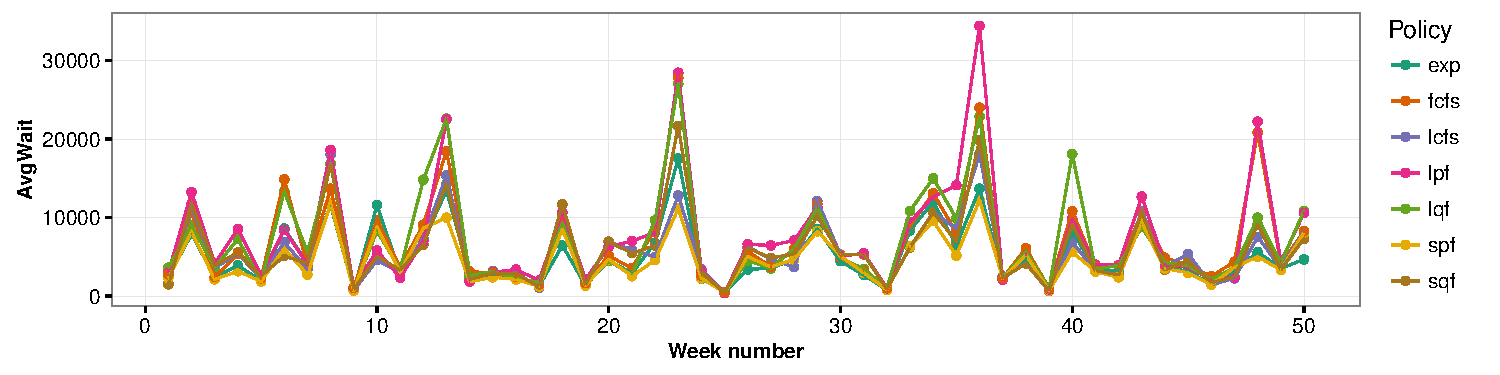
\includegraphics[scale=0.6]{variability.pdf}
  \caption{Variability in the weekly average waiting time in the KTH-SP2 trace (pre-processing described in subsection~\ref{sub:traces}) for a few policies.}
  \label{fig:mosn}
\end{figure*}

%Validating algorithms on real data is a notoriously hard
%problem~\cite{feitbook}. The case of batch scheduling is made especially
%difficult by the fluctuations in commonly used metrics~\cite{jsm}. Indeed, the
%variability in performance is known to outrank the available sample sizes:
%\textit{It is not enough to simply replay an algorithm using a trace}. For this
%reason, we clearly expose our statistical approach.

%Two main methods are available in order to generate data. On one hand, it is
%possible to model~\cite{feitperfeval} workloads. However, this often loses
%many specificities of the original data, and this work uses a second
%approach based on trace resampling~\cite{feitresampling}.

To carry our experiments, we need to generate many trace samples. More precisely, we want
to sample the job submission process, which is achieved by splitting the traces in weeks,
randomly shuffling them and picking the jobs submitted in the selected weeks.  This simple
mechanism enables us to preserve the dependency within a week. Although the system state
may not be independent from one week to an other, we can reasonably assume that it evolves
under its stationary distribution. Thus, computing an average over the sampled traces at a
given time can be related to a time average of an underlying Markov process, which
converges to the true quantity thanks to the ergodic theorem.  Moreover, the job
submission process has no long range correlation making it look like an independent and
identically distributed process when considering sufficiently time spaced weeks.

\subsubsection{Experimental campaign}


\subsubsection{Replicability}

Readers interested in replicating the experiments (or a part thereof) are
invited to peruse to the 'artifacts description' appendix of this paper.  We
provide to persistent archives containing the simulator used, the analysis code
and the associated workflow necessary to replicate all experiments and figures
present in this paper. All these parts's dependencies are automatically managed
via Nix~\cite{nix} and we invite the reader to replicate the results.

\subsection{Results}
\label{sub:results}

\begin{figure*}[h]
  \centering
  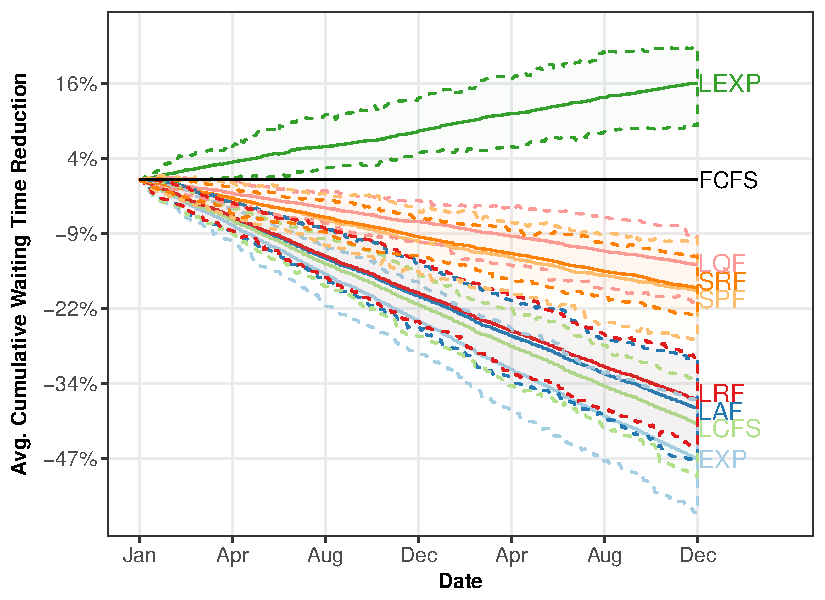
\includegraphics[scale=0.6]{full-CTC-SP2.pdf}
  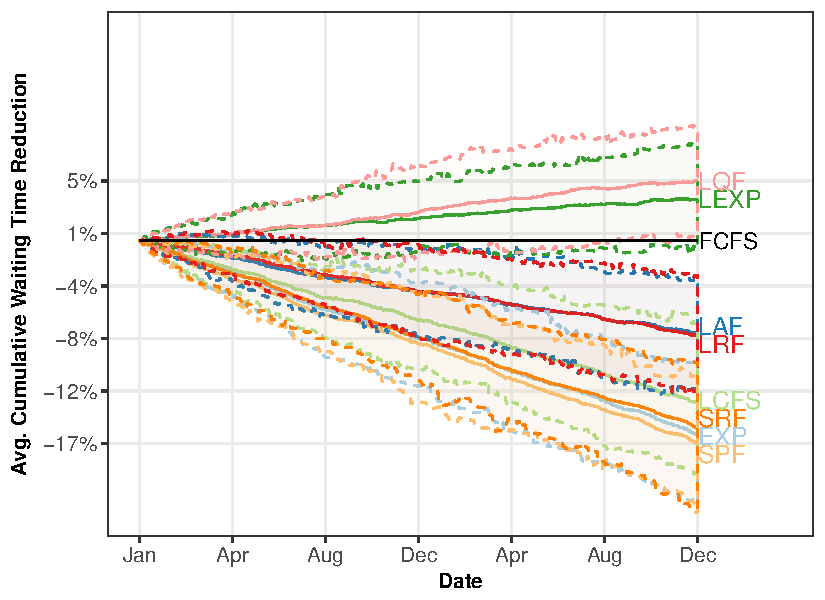
\includegraphics[scale=0.6]{full-KTH-SP2.pdf}\\
  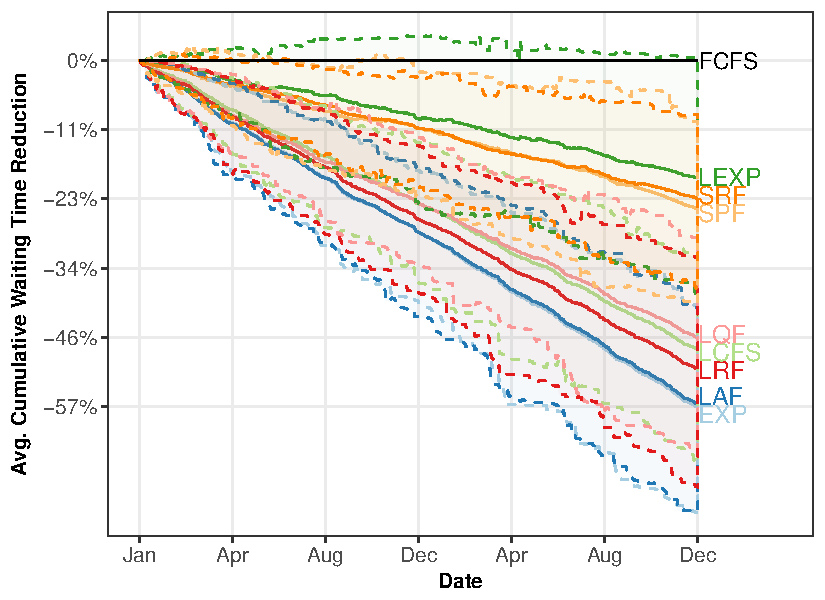
\includegraphics[scale=0.6]{full-CEA-Curi.pdf}
  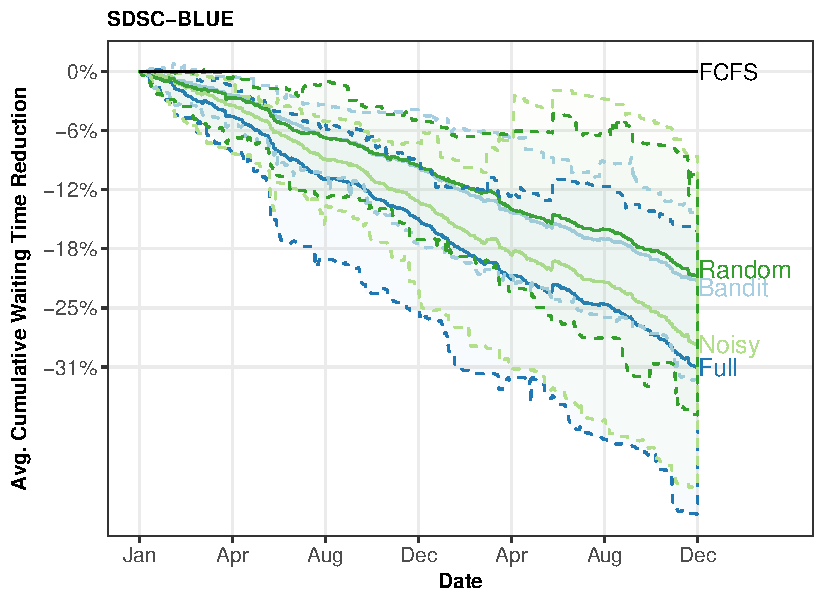
\includegraphics[scale=0.6]{full-SDSC-BLU.pdf}\\
  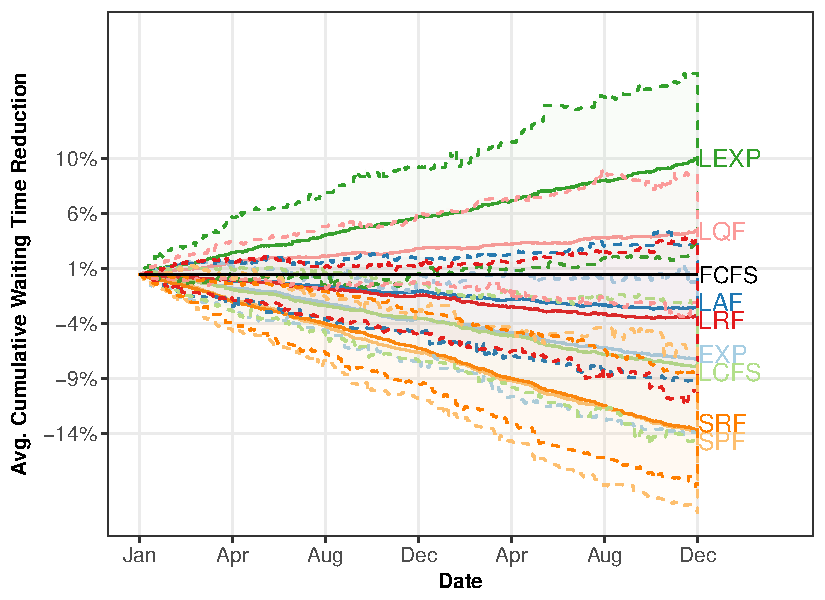
\includegraphics[scale=0.6]{full-SDSC-SP2.pdf}
  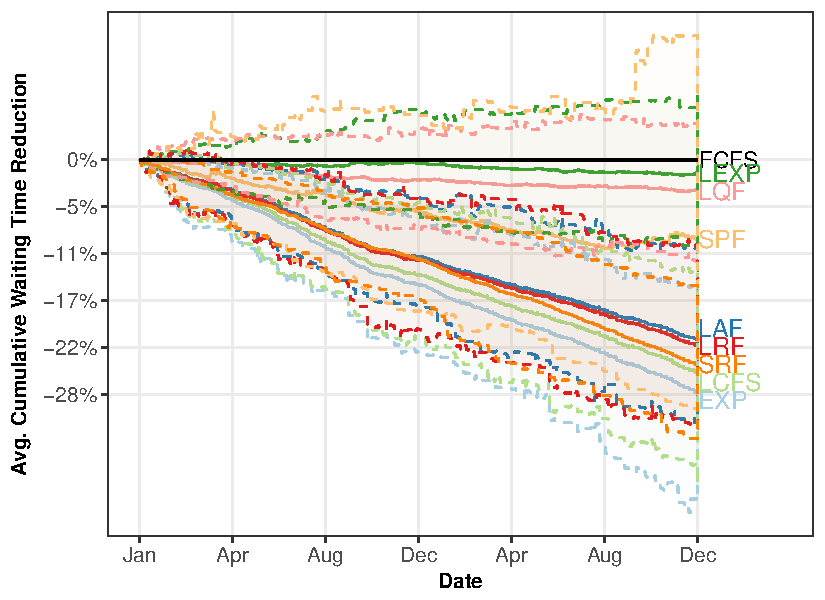
\includegraphics[scale=0.6]{full-ANL-Intr.pdf}

  \caption{Evolution of the average cumulative waiting time improvement
    compared to EASY-FCFS of the FullFeedback, NoisyFeedback and EpsilonGreedy
    policies. The average is obtained by resampling the original trace 100
    times. The dashed lines represent the 10th and 90th percentiles of the
  values across this resampling. Each figure is a different trace, and this
figure is followed-up in figure~\ref{fig:follow} for the UniLu-Gaia log.}

  \label{fig:small}
\end{figure*}

\begin{figure}[ht]
  \centering
  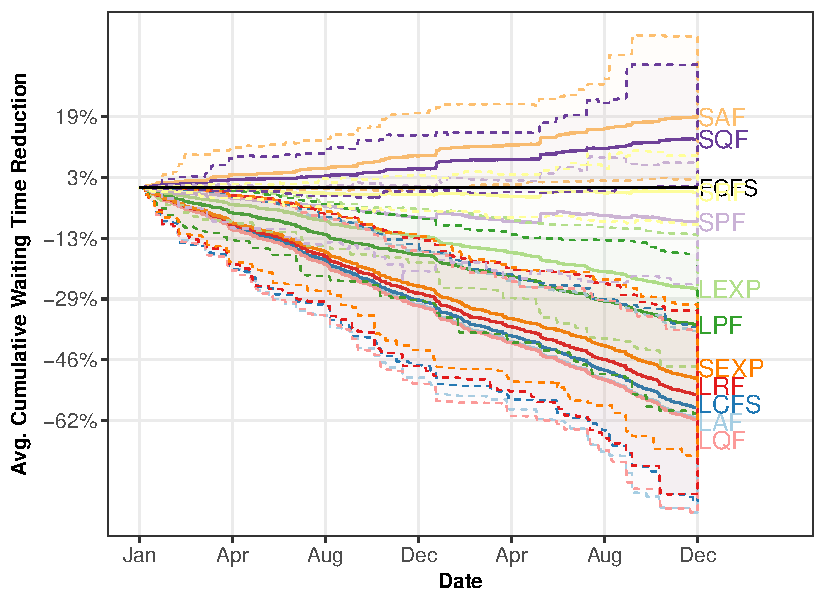
\includegraphics[scale=0.6]{full-UniLu-Ga.pdf}

  \caption{Follow-up from figure~\ref{fig:small}, plot for the UniLu-Gaia log.}

  \label{fig:follow}
\end{figure}

\begin{figure}[H]
  \centering
  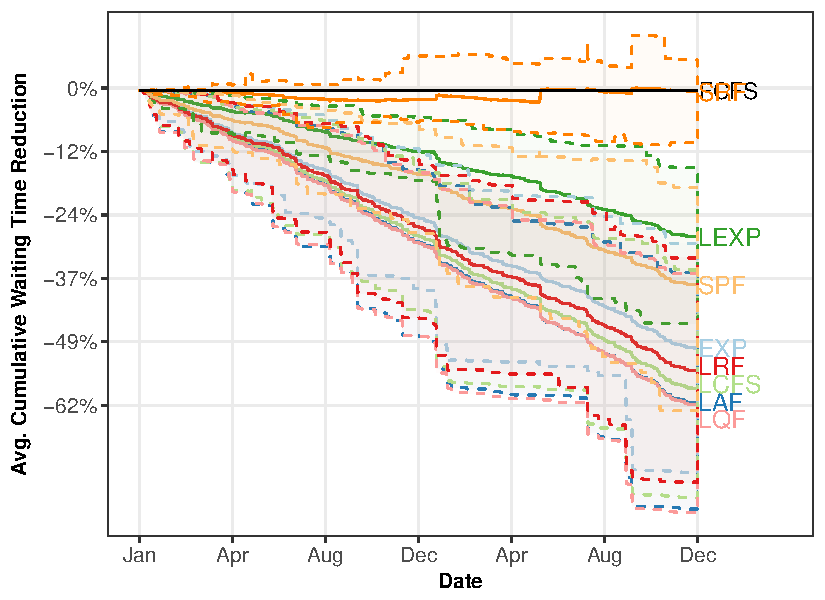
\includegraphics[scale=0.6]{UniLu-Ga.pdf}

  \caption{Evolution of the average cumulative waiting time improvement
    compared to EASY-FCFS of the policies $P_i$ for $i = 1 \ldots 10$. The
    average is obtained by resampling the original trace 100 times. The dashed
    lines represent the 10th and 90th percentiles of the values across this
  resampling. Each figure is a different trace, and this figure is followed-up
in figure~\ref{fig:follow} for the UniLu-Gaia log.}

  \label{fig:all}
\end{figure}

\begin{figure}[H]
  \centering
  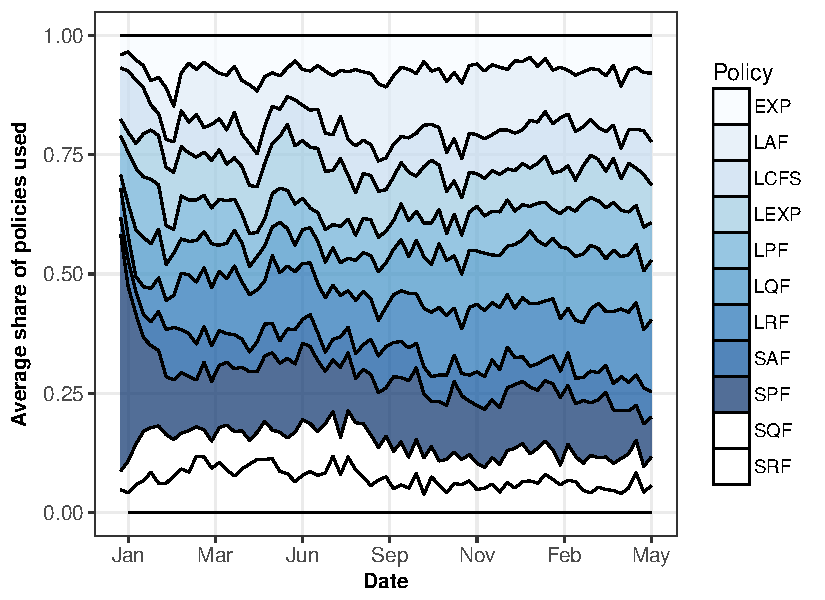
\includegraphics[scale=0.6]{mosaicbandit-UniLu-Ga.pdf}
  \caption{Share of the policies chosen by Epsilon-Greedy as a function of time.
  The average choice is obtained by resampling the original trace 100 times and
  aggregating by date.}
  \label{fig:mosb}
\end{figure}

\begin{figure}[ht]
  \centering
  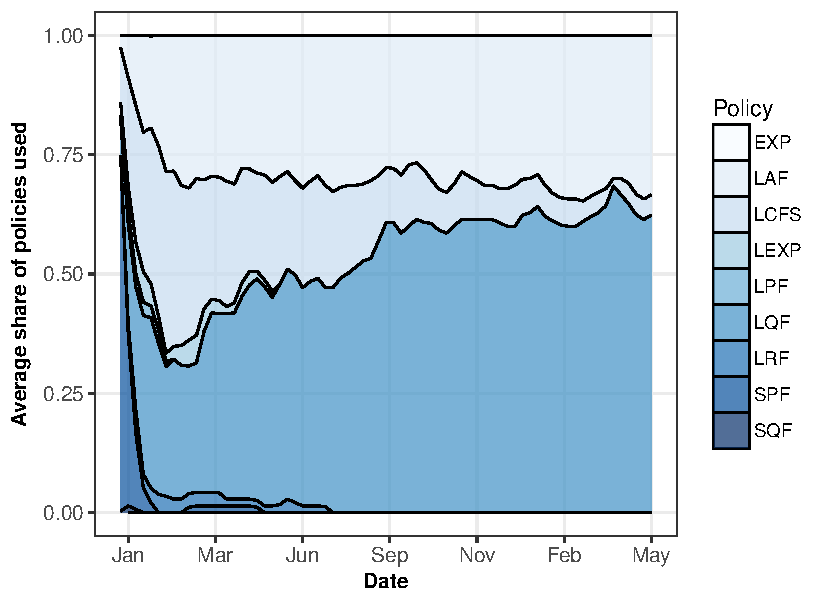
\includegraphics[scale=0.6]{mosaic-UniLu-Ga.pdf}
  \caption{Share of the policies chosen by the Noisy policy. The average
  choice is obtained by resampling the original trace 100 times and
  aggregating by date.}
  \label{fig:mosn}
\end{figure}

\section{Conclusion}
\label{sec:ccl}

\begin{acks}

Authors are sorted in alphabetical order. We gracefully thank the contributors
of the Parallel Workloads Archive, Victor Hazlewood (SDSC SP2), Travis Earheart
and Nancy Wilkins-Diehr (SDSC Blue), Lars Malinowsky (KTH SP2), Dan Dwyer and
Steve Hotovy (CTC SP2), Joseph Emeras (CEA Curie and UniLu Gaia), Susan
Coghlan, Narayan Desay, Wei Tang (ANL Intrepid), and of course Dror Feitelson.
The Metacentrum workload log was graciously provided by the Czech National Grid
Infrastructure MetaCentrum. This work has been partially supported by the LabEx
PERSYVAL-Lab(\grantsponsor{ANR-11-LABX-0025-01}{ANR-11-LABX-0025-01}) funded by
the French program Investissement d'avenir. Experiments presented in this paper
were carried out using the Grid'5000 testbed. Grid'5000 is supported by a
scientific interest group hosted by Inria and including CNRS, RENATER and
several Universities as well as other
organizations\footnote{https://www.grid5000.fr}.  Access to the experimental
machine(s) used in this paper was gracefully granted by research teams from
LIG\footnote{http://www.liglab.fr} and Inria\footnote{http://www.inria.fr}.

\end{acks}

\bibliographystyle{acmst}
\bibliography{bibliography}

\clearpage
\section*{Artifacts Description}

We develop a lightweight simulator~\cite{ocst} and an accompanying multi-armed
bandit library~\cite{obandit}. Both are made available under the ISC~\cite{isc}
license and released as persistent Zenodo~\cite{zenodo} archives. Additionally,
we provide a workflow written in the zymake~\cite{breck2008zymake} format that
is able to generate all the figures from this paper and its annexes. All these
parts and their dependencies are packaged via Nix~\cite{nix} expressions.
to use the
archive at~\cite{repro} on any linux system equipped with the Nix package manager.
Generating the figures is done with:

\begin{lstlisting}
wget ".." -o banditeasy.tgz
tar -vzf banditeasy.tgz
cd banditeasy
nix-build
\end{lstlisting}


\end{document}
